\chapter{强连通性}

\index{强连通图}

在有向图中，
边只能沿一个方向遍历，
因此即使图是连通的，
这也不能保证从一个节点可以到达另一个节点。
出于这个原因，定义一个比连通性要求更高的新概念是有意义的。

如果一个图是\key{强连通的}，
则图中存在从任意节点到所有其他节点的路径。
例如，在下图中，
左图是强连通的，
而右图不是。

\begin{center}
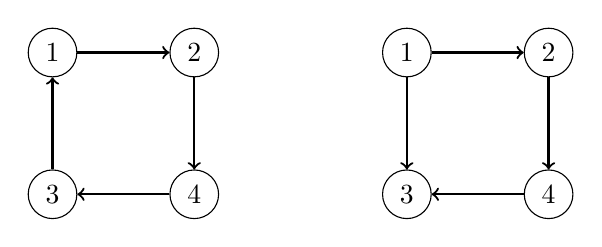
\begin{tikzpicture}[scale=0.9]
\node[draw, circle] (1) at (1,1) {$1$};
\node[draw, circle] (2) at (3,1) {$2$};
\node[draw, circle] (3) at (1,-1) {$3$};
\node[draw, circle] (4) at (3,-1) {$4$};

\path[draw,thick,->] (1) -- (2);
\path[draw,thick,->] (2) -- (4);
\path[draw,thick,->] (4) -- (3);
\path[draw,thick,->] (3) -- (1);

\node[draw, circle] (1b) at (6,1) {$1$};
\node[draw, circle] (2b) at (8,1) {$2$};
\node[draw, circle] (3b) at (6,-1) {$3$};
\node[draw, circle] (4b) at (8,-1) {$4$};

\path[draw,thick,->] (1b) -- (2b);
\path[draw,thick,->] (2b) -- (4b);
\path[draw,thick,->] (4b) -- (3b);
\path[draw,thick,->] (1b) -- (3b);
\end{tikzpicture}
\end{center}

右图不是强连通的，
因为例如不存在
从节点2到节点1的路径。

\index{强连通分量}
\index{分量图}

图的\key{强连通分量}将图划分为
尽可能大的强连通部分。
强连通分量构成一个无环的\key{分量图}，
表示原图的深层结构。

例如，对于图
\begin{center}
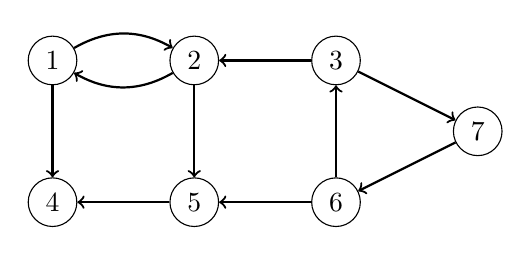
\begin{tikzpicture}[scale=0.9,label distance=-2mm]
\node[draw, circle] (1) at (-1,1) {$7$};
\node[draw, circle] (2) at (-3,2) {$3$};
\node[draw, circle] (4) at (-5,2) {$2$};
\node[draw, circle] (6) at (-7,2) {$1$};
\node[draw, circle] (3) at (-3,0) {$6$};
\node[draw, circle] (5) at (-5,0) {$5$};
\node[draw, circle] (7) at (-7,0) {$4$};

\path[draw,thick,->] (2) -- (1);
\path[draw,thick,->] (1) -- (3);
\path[draw,thick,->] (3) -- (2);
\path[draw,thick,->] (2) -- (4);
\path[draw,thick,->] (3) -- (5);
\path[draw,thick,->] (4) edge [bend left] (6);
\path[draw,thick,->] (6) edge [bend left] (4);
\path[draw,thick,->] (4) -- (5);
\path[draw,thick,->] (5) -- (7);
\path[draw,thick,->] (6) -- (7);
\end{tikzpicture}
\end{center}
其强连通分量如下：
\begin{center}
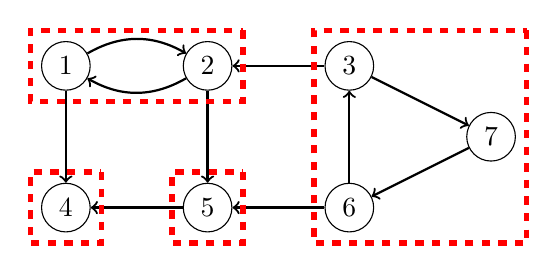
\begin{tikzpicture}[scale=0.9]
\node[draw, circle] (1) at (-1,1) {$7$};
\node[draw, circle] (2) at (-3,2) {$3$};
\node[draw, circle] (4) at (-5,2) {$2$};
\node[draw, circle] (6) at (-7,2) {$1$};
\node[draw, circle] (3) at (-3,0) {$6$};
\node[draw, circle] (5) at (-5,0) {$5$};
\node[draw, circle] (7) at (-7,0) {$4$};

\path[draw,thick,->] (2) -- (1);
\path[draw,thick,->] (1) -- (3);
\path[draw,thick,->] (3) -- (2);
\path[draw,thick,->] (2) -- (4);
\path[draw,thick,->] (3) -- (5);
\path[draw,thick,->] (4) edge [bend left] (6);
\path[draw,thick,->] (6) edge [bend left] (4);
\path[draw,thick,->] (4) -- (5);
\path[draw,thick,->] (5) -- (7);
\path[draw,thick,->] (6) -- (7);

\draw [red,thick,dashed,line width=2pt] (-0.5,2.5) rectangle (-3.5,-0.5);
\draw [red,thick,dashed,line width=2pt] (-4.5,2.5) rectangle (-7.5,1.5);
\draw [red,thick,dashed,line width=2pt] (-4.5,0.5) rectangle (-5.5,-0.5);
\draw [red,thick,dashed,line width=2pt] (-6.5,0.5) rectangle (-7.5,-0.5);
\end{tikzpicture}
\end{center}
对应的分量图如下：
\begin{center}
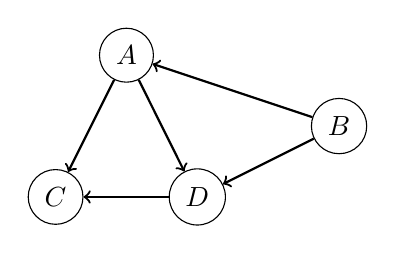
\begin{tikzpicture}[scale=0.9]
\node[draw, circle] (1) at (-3,1) {$B$};
\node[draw, circle] (2) at (-6,2) {$A$};
\node[draw, circle] (3) at (-5,0) {$D$};
\node[draw, circle] (4) at (-7,0) {$C$};

\path[draw,thick,->] (1) -- (2);
\path[draw,thick,->] (1) -- (3);
\path[draw,thick,->] (2) -- (3);
\path[draw,thick,->] (2) -- (4);
\path[draw,thick,->] (3) -- (4);
\end{tikzpicture}
\end{center}
各分量为 $A=\{1,2\}$,
$B=\{3,6,7\}$，$C=\{4\}$ 和 $D=\{5\}$。

分量图是一个无环有向图，
因此它比原图更容易处理。
由于图中不包含环，
我们总是可以构造一个拓扑排序，
并使用第16章中介绍的动态规划技术。

\section{Kosaraju算法}

\index{Kosaraju算法}

\key{Kosaraju算法}\footnote{根据 \cite{aho83}，
S. R. Kosaraju 于1978年发明了这个算法
但未发表。1981年，同样的算法被 M. Sharir \cite{sha81} 重新发现并发表。}
是一种寻找有向图强连通分量的高效方法。
该算法执行两次深度优先搜索：
第一次搜索根据图的结构构造节点列表，
第二次搜索形成强连通分量。

\subsubsection{搜索1}

Kosaraju算法的第一阶段构造一个节点列表，
列表顺序为深度优先搜索处理节点的顺序。
算法遍历所有节点，
并在每个未处理的节点处开始一次深度优先搜索。
每个节点在被处理完后会被添加到列表中。

在示例图中，节点按以下顺序被处理：
\begin{center}
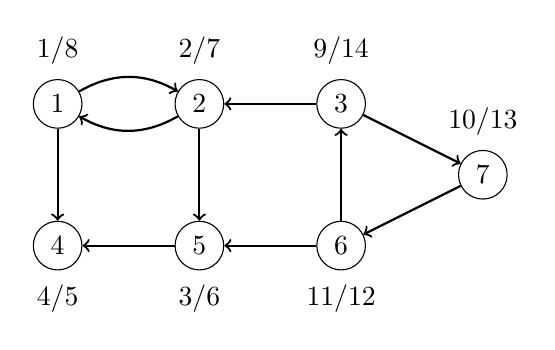
\begin{tikzpicture}[scale=0.9,label distance=-2mm]
\node[draw, circle] (1) at (-1,1) {$7$};
\node[draw, circle] (2) at (-3,2) {$3$};
\node[draw, circle] (4) at (-5,2) {$2$};
\node[draw, circle] (6) at (-7,2) {$1$};
\node[draw, circle] (3) at (-3,0) {$6$};
\node[draw, circle] (5) at (-5,0) {$5$};
\node[draw, circle] (7) at (-7,0) {$4$};

\node at (-7,2.75) {$1/8$};
\node at (-5,2.75) {$2/7$};
\node at (-3,2.75) {$9/14$};
\node at (-7,-0.75) {$4/5$};
\node at (-5,-0.75) {$3/6$};
\node at (-3,-0.75) {$11/12$};
\node at (-1,1.75) {$10/13$};

\path[draw,thick,->] (2) -- (1);
\path[draw,thick,->] (1) -- (3);
\path[draw,thick,->] (3) -- (2);
\path[draw,thick,->] (2) -- (4);
\path[draw,thick,->] (3) -- (5);
\path[draw,thick,->] (4) edge [bend left] (6);
\path[draw,thick,->] (6) edge [bend left] (4);
\path[draw,thick,->] (4) -- (5);
\path[draw,thick,->] (5) -- (7);
\path[draw,thick,->] (6) -- (7);
\end{tikzpicture}
\end{center}

记号 $x/y$ 表示
节点的处理在时间 $x$ 开始，
在时间 $y$ 结束。
因此，对应的列表如下：

\begin{tabular}{ll}
\\
节点 & 处理时间 \\
\hline
4 & 5 \\
5 & 6 \\
2 & 7 \\
1 & 8 \\
6 & 12 \\
7 & 13 \\
3 & 14 \\
\\
\end{tabular}
% 
% In the second phase of the algorithm,
% the nodes will be processed
% in reverse order: $[3,7,6,1,2,5,4]$.

\subsubsection{搜索2}

算法的第二阶段
形成图的强连通分量。
首先，算法反转图中的每条边。
这保证了在第二次搜索中，
我们总能找到不包含多余节点的
强连通分量。

反转边后，
示例图如下：
\begin{center}
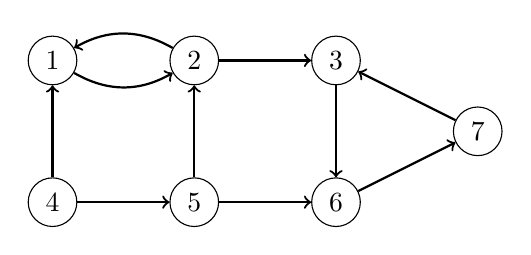
\begin{tikzpicture}[scale=0.9,label distance=-2mm]
\node[draw, circle] (1) at (-1,1) {$7$};
\node[draw, circle] (2) at (-3,2) {$3$};
\node[draw, circle] (4) at (-5,2) {$2$};
\node[draw, circle] (6) at (-7,2) {$1$};
\node[draw, circle] (3) at (-3,0) {$6$};
\node[draw, circle] (5) at (-5,0) {$5$};
\node[draw, circle] (7) at (-7,0) {$4$};

\path[draw,thick,<-] (2) -- (1);
\path[draw,thick,<-] (1) -- (3);
\path[draw,thick,<-] (3) -- (2);
\path[draw,thick,<-] (2) -- (4);
\path[draw,thick,<-] (3) -- (5);
\path[draw,thick,<-] (4) edge [bend left] (6);
\path[draw,thick,<-] (6) edge [bend left] (4);
\path[draw,thick,<-] (4) -- (5);
\path[draw,thick,<-] (5) -- (7);
\path[draw,thick,<-] (6) -- (7);
\end{tikzpicture}
\end{center}

之后，算法按第一次搜索创建的节点列表
以\emph{逆序}遍历。
如果一个节点不属于任何分量，
算法会创建一个新分量，
并开始一次深度优先搜索，
将搜索过程中发现的所有新节点
添加到新分量中。

在示例图中，第一个分量
从节点3开始：

\begin{center}
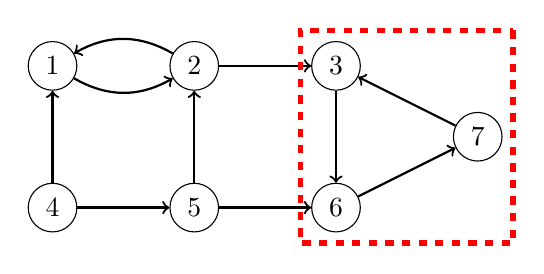
\begin{tikzpicture}[scale=0.9,label distance=-2mm]
\node[draw, circle] (1) at (-1,1) {$7$};
\node[draw, circle] (2) at (-3,2) {$3$};
\node[draw, circle] (4) at (-5,2) {$2$};
\node[draw, circle] (6) at (-7,2) {$1$};
\node[draw, circle] (3) at (-3,0) {$6$};
\node[draw, circle] (5) at (-5,0) {$5$};
\node[draw, circle] (7) at (-7,0) {$4$};

\path[draw,thick,<-] (2) -- (1);
\path[draw,thick,<-] (1) -- (3);
\path[draw,thick,<-] (3) -- (2);
\path[draw,thick,<-] (2) -- (4);
\path[draw,thick,<-] (3) -- (5);
\path[draw,thick,<-] (4) edge [bend left] (6);
\path[draw,thick,<-] (6) edge [bend left] (4);
\path[draw,thick,<-] (4) -- (5);
\path[draw,thick,<-] (5) -- (7);
\path[draw,thick,<-] (6) -- (7);

\draw [red,thick,dashed,line width=2pt] (-0.5,2.5) rectangle (-3.5,-0.5);
\end{tikzpicture}
\end{center}

注意，由于所有边都被反转，
该分量不会“泄漏”到图中的其他部分。

\begin{samepage}
列表中的下一个节点是节点7和6，
但它们已经属于一个分量，
因此下一个新分量从节点1开始：

\begin{center}
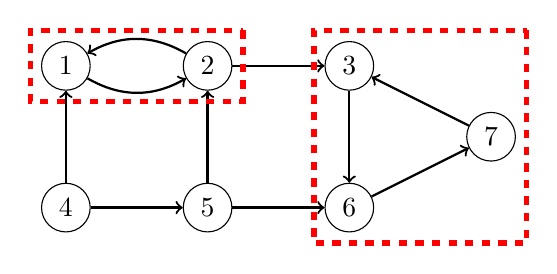
\begin{tikzpicture}[scale=0.9,label distance=-2mm]
\node[draw, circle] (1) at (-1,1) {$7$};
\node[draw, circle] (2) at (-3,2) {$3$};
\node[draw, circle] (4) at (-5,2) {$2$};
\node[draw, circle] (6) at (-7,2) {$1$};
\node[draw, circle] (3) at (-3,0) {$6$};
\node[draw, circle] (5) at (-5,0) {$5$};
\node[draw, circle] (7) at (-7,0) {$4$};

\path[draw,thick,<-] (2) -- (1);
\path[draw,thick,<-] (1) -- (3);
\path[draw,thick,<-] (3) -- (2);
\path[draw,thick,<-] (2) -- (4);
\path[draw,thick,<-] (3) -- (5);
\path[draw,thick,<-] (4) edge [bend left] (6);
\path[draw,thick,<-] (6) edge [bend left] (4);
\path[draw,thick,<-] (4) -- (5);
\path[draw,thick,<-] (5) -- (7);
\path[draw,thick,<-] (6) -- (7);

\draw [red,thick,dashed,line width=2pt] (-0.5,2.5) rectangle (-3.5,-0.5);
\draw [red,thick,dashed,line width=2pt] (-4.5,2.5) rectangle (-7.5,1.5);
%\draw [red,thick,dashed,line width=2pt] (-4.5,0.5) rectangle (-5.5,-0.5);
%\draw [red,thick,dashed,line width=2pt] (-6.5,0.5) rectangle (-7.5,-0.5);
\end{tikzpicture}
\end{center}
\end{samepage}

\begin{samepage}
最后，算法处理节点5和4，
它们构成剩余的强连通分量：

\begin{center}
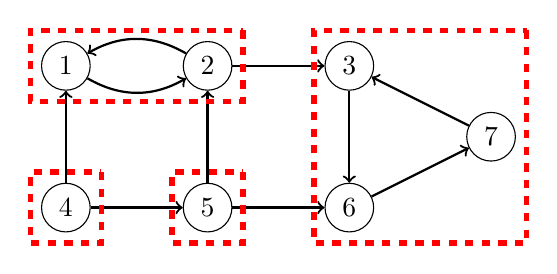
\begin{tikzpicture}[scale=0.9,label distance=-2mm]
\node[draw, circle] (1) at (-1,1) {$7$};
\node[draw, circle] (2) at (-3,2) {$3$};
\node[draw, circle] (4) at (-5,2) {$2$};
\node[draw, circle] (6) at (-7,2) {$1$};
\node[draw, circle] (3) at (-3,0) {$6$};
\node[draw, circle] (5) at (-5,0) {$5$};
\node[draw, circle] (7) at (-7,0) {$4$};

\path[draw,thick,<-] (2) -- (1);
\path[draw,thick,<-] (1) -- (3);
\path[draw,thick,<-] (3) -- (2);
\path[draw,thick,<-] (2) -- (4);
\path[draw,thick,<-] (3) -- (5);
\path[draw,thick,<-] (4) edge [bend left] (6);
\path[draw,thick,<-] (6) edge [bend left] (4);
\path[draw,thick,<-] (4) -- (5);
\path[draw,thick,<-] (5) -- (7);
\path[draw,thick,<-] (6) -- (7);

\draw [red,thick,dashed,line width=2pt] (-0.5,2.5) rectangle (-3.5,-0.5);
\draw [red,thick,dashed,line width=2pt] (-4.5,2.5) rectangle (-7.5,1.5);
\draw [red,thick,dashed,line width=2pt] (-4.5,0.5) rectangle (-5.5,-0.5);
\draw [red,thick,dashed,line width=2pt] (-6.5,0.5) rectangle (-7.5,-0.5);
\end{tikzpicture}
\end{center}
\end{samepage}

该算法的时间复杂度为 $O(n+m)$，
因为算法执行两次深度优先搜索。

\section{2SAT问题}

\index{2SAT问题}

强连通性也与
\key{2SAT问题}\footnote{这里介绍的算法是在 \cite{asp79} 中提出的。
还有另一种著名的线性时间算法 \cite{eve75}，
它基于回溯。}有关。
在这个问题中，给定一个逻辑公式
\[
(a_1 \lor b_1) \land (a_2 \lor b_2) \land \cdots \land (a_m \lor b_m),
\]
其中每个 $a_i$ 和 $b_i$ 是一个逻辑变量
($x_1,x_2,\ldots,x_n$)
或一个逻辑变量的否定
($\lnot x_1, \lnot x_2, \ldots, \lnot x_n$)。
符号“$\land$”和“$\lor$”分别表示
逻辑运算符“与”和“或”。
我们的任务是为每个变量赋值，
使公式为真，或者说明这不可能。

例如，公式
\[
L_1 = (x_2 \lor \lnot x_1) \land
      (\lnot x_1 \lor \lnot x_2) \land
      (x_1 \lor x_3) \land
      (\lnot x_2 \lor \lnot x_3) \land
      (x_1 \lor x_4)
\]
在变量如下赋值时为真：

\[
\begin{cases}
x_1 = \textrm{false} \\
x_2 = \textrm{false} \\
x_3 = \textrm{true} \\
x_4 = \textrm{true} \\
\end{cases}
\]

然而，公式
\[
L_2 = (x_1 \lor x_2) \land
      (x_1 \lor \lnot x_2) \land
      (\lnot x_1 \lor x_3) \land
      (\lnot x_1 \lor \lnot x_3)
\]
总是为假的，无论我们如何赋值。
原因是我们不能
为 $x_1$ 选择一个值
而不产生矛盾。
如果 $x_1$ 为假，则 $x_2$ 和 $\lnot x_2$
都应为真，这是不可能的；
如果 $x_1$ 为真，则 $x_3$ 和 $\lnot x_3$
都应为真，这也是不可能的。

2SAT问题可以表示为一个图，
其节点对应于
变量 $x_i$ 和否定 $\lnot x_i$，
边确定了变量之间的连接。
每个对 $(a_i \lor b_i)$ 生成两条边：
$\lnot a_i \to b_i$ 和 $\lnot b_i \to a_i$。
这意味着如果 $a_i$ 不成立，
则 $b_i$ 必须成立，反之亦然。

公式 $L_1$ 的图为：
\\
\begin{center}
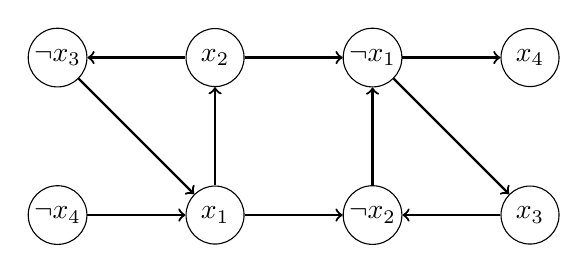
\begin{tikzpicture}[scale=1.0,minimum size=2pt]
\node[draw, circle, inner sep=1.3pt] (1) at (1,2) {$\lnot x_3$};
\node[draw, circle] (2) at (3,2) {$x_2$};
\node[draw, circle, inner sep=1.3pt] (3) at (1,0) {$\lnot x_4$};
\node[draw, circle] (4) at (3,0) {$x_1$};
\node[draw, circle, inner sep=1.3pt] (5) at (5,2) {$\lnot x_1$};
\node[draw, circle] (6) at (7,2) {$x_4$};
\node[draw, circle, inner sep=1.3pt] (7) at (5,0) {$\lnot x_2$};
\node[draw, circle] (8) at (7,0) {$x_3$};
 
\path[draw,thick,->] (1) -- (4);
\path[draw,thick,->] (4) -- (2);
\path[draw,thick,->] (2) -- (1);
\path[draw,thick,->] (3) -- (4);
\path[draw,thick,->] (2) -- (5);
\path[draw,thick,->] (4) -- (7);
\path[draw,thick,->] (5) -- (6);
\path[draw,thick,->] (5) -- (8);
\path[draw,thick,->] (8) -- (7);
\path[draw,thick,->] (7) -- (5);
\end{tikzpicture}
\end{center}
公式 $L_2$ 的图为：
\\
\begin{center}
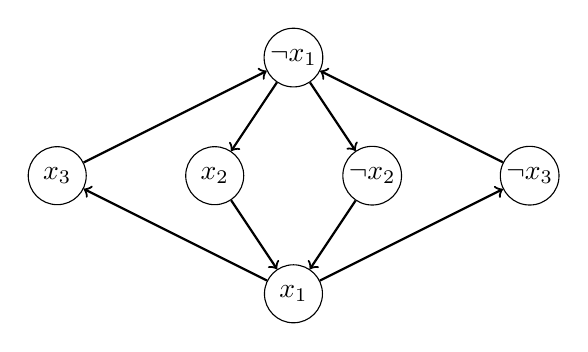
\begin{tikzpicture}[scale=1.0,minimum size=2pt]
\node[draw, circle] (1) at (1,2) {$x_3$};
\node[draw, circle] (2) at (3,2) {$x_2$};
\node[draw, circle, inner sep=1.3pt] (3) at (5,2) {$\lnot x_2$};
\node[draw, circle, inner sep=1.3pt] (4) at (7,2) {$\lnot x_3$};
\node[draw, circle, inner sep=1.3pt] (5) at (4,3.5) {$\lnot x_1$};
\node[draw, circle] (6) at (4,0.5) {$x_1$};

\path[draw,thick,->] (1) -- (5);
\path[draw,thick,->] (4) -- (5);
\path[draw,thick,->] (6) -- (1);
\path[draw,thick,->] (6) -- (4);
\path[draw,thick,->] (5) -- (2);
\path[draw,thick,->] (5) -- (3);
\path[draw,thick,->] (2) -- (6);
\path[draw,thick,->] (3) -- (6);
\end{tikzpicture}
\end{center}

图的结构告诉我们
是否可以为变量赋值
使公式为真。
结果表明，当且仅当不存在
节点 $x_i$ 和 $\lnot x_i$ 同时属于
同一个强连通分量时，这是可以做到的。
如果存在这样的节点，
则图中包含
从 $x_i$ 到 $\lnot x_i$ 的路径，
也包含从 $\lnot x_i$ 到 $x_i$ 的路径，
因此 $x_i$ 和 $\lnot x_i$ 都应为真，
这是不可能的。

在公式 $L_1$ 的图中
不存在节点 $x_i$ 和 $\lnot x_i$
同时属于同一个强连通分量，
因此存在解。
在公式 $L_2$ 的图中
所有节点属于同一个强连通分量，
因此不存在解。

如果存在解，可以通过以逆拓扑排序顺序遍历
分量图的节点来找到变量的值。
在每一步中，我们处理一个
不包含指向未处理分量的边的分量。
如果分量中的变量
尚未被赋值，
则其值将根据分量中的值来确定；
如果已经有值，则保持不变。
该过程持续进行，直到每个变量
都被赋值。

公式 $L_1$ 的分量图如下：
\begin{center}
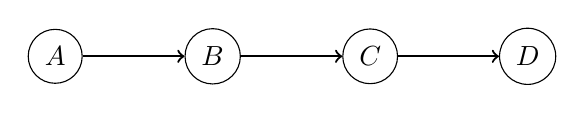
\begin{tikzpicture}[scale=1.0]
\node[draw, circle] (1) at (0,0) {$A$};
\node[draw, circle] (2) at (2,0) {$B$};
\node[draw, circle] (3) at (4,0) {$C$};
\node[draw, circle] (4) at (6,0) {$D$};

\path[draw,thick,->] (1) -- (2);
\path[draw,thick,->] (2) -- (3);
\path[draw,thick,->] (3) -- (4);
\end{tikzpicture}
\end{center}

各分量为
$A = \{\lnot x_4\}$，
$B = \{x_1, x_2, \lnot x_3\}$，
$C = \{\lnot x_1, \lnot x_2, x_3\}$ 和
$D = \{x_4\}$。
构造解时，
我们首先处理分量 $D$，
其中 $x_4$ 变为真。
之后，我们处理分量 $C$，
其中 $x_1$ 和 $x_2$ 变为假，
$x_3$ 变为真。
所有变量都已被赋值，
因此剩余的分量 $A$ 和 $B$
不会改变变量。

注意这种方法有效，因为
图具有特殊的结构：
如果存在从节点 $x_i$ 到节点 $x_j$ 的路径
以及从节点 $x_j$ 到节点 $\lnot x_j$ 的路径，
则节点 $x_i$ 永远不会变为真。
原因是还存在
从节点 $\lnot x_j$ 到节点 $\lnot x_i$ 的路径，
并且 $x_i$ 和 $x_j$ 都变为假。

\index{3SAT问题}

更难的问题是\key{3SAT问题}，
其中公式的每个部分形式为
$(a_i \lor b_i \lor c_i)$。
这个问题是NP难的，因此没有已知的高效算法来求解。
